\subsection{Protocol Selection}

\subsubsection{Requirements}
    \paragraph{Flight Controller}
    The flight controller and its associated devices are the core of the communication network as it connects all the devices required to fly. Table \ref{tab:device_comms_requirementsl} shows the messages that interact with the flight controller. As these messages are significantly smaller than the main sensor messages they will be considered separately. The net bandwidth required is \textbf{do the math} using 64 bit messages.
    \gls{BMS}
    \gls{GNSS}
    \begin{table}[]
        \begin{tabular}{|c|c|c|c|c|c|} 
         \textbf{Source}             & \textbf{Target}            & \textbf{Quantity}   & \textbf{Purpose}& \textbf{Frequency} & \textbf{Bandwidth}\\
         \hline
         Flight Controller  & \gls{ESC}         & 4    & Duty Cycle        & 400 Hz & 51.2 kbps \\
         Flight Controller  & On Board Computer & 1    & Longitude         & 10 Hz  & 51.2 kbps \\
         Flight Controller  & On Board Computer & 1    & Latitude         & 10 Hz   & 51.2 kbps \\
         Flight Controller  & On Board Computer & 1    & Altitude         & 10 Hz   & 51.2 kbps \\
         On Board Computer  & Flight Controller & 1    & Desired Longitude & 1 Hz & 51.2 kbps \\
         On Board Computer  & Flight Controller & 1    & Desired Latitude & 1 Hz      & 51.2 kbps \\
         On Board Computer  & Flight Controller & 1    & Desired Altitude & 1 Hz   & 51.2 kbps \\
         \gls{ESC}          & Flight Controller & 4    & \gls{RPM}         & 10 Hz     & 1.28 kbps \\
         \gls{ESC}          & Flight Controller & 4    & Current           & 10 Hz     & 1.28 kbps \\
         \gls{ESC}          & Flight Controller & 4    & Voltage           & 10 Hz     & 1.28 kbps \\
         \gls{ESC}          & Flight Controller & 4    & \gls{ESC} Temperature & 1 Hz    & 0.128 kbps \\
         \gls{BMS}          & Flight Controller & 1    & State of Charge & 1 Hz     & 0.032 kbps \\
         \gls{BMS}          & Flight Controller & 1    & Battery temperature & 1 Hz     & 0.128 kbps \\
         \gls{GNSS} module  & Flight Controller & 2    & Longitude  & 1 Hz       & 0.064 kbps \\
         \gls{GNSS} module  & Flight Controller & 2    & Latitude   & 1 Hz     & 0.064 kbps \\
         \gls{GNSS} module  & Flight Controller & 2    & Altitude   & 1 Hz      & 0.064 kbps \\
         Collision detection  & Flight Controller & 2    & Collision detect  & 10 Hz     & 0.64 kbps \\
         Collision detection& Flight Controller & 2    & Altitude  & 10 Hz      & 0.64 kbps \\
         \hline
        \end{tabular}
        \caption{Required Messages}
        \label{tab:device_comms_requirementsl}
    \end{table}
    
\subsubsection{Options}
\begin{table}[]
        \centering
        \begin{tabular}{|c|c|c|c|c|c|c|} 
         \textbf{Protocol} & \textbf{Speed} & \textbf{Complexity} &\textbf{Power Draw} &\textbf{Noise tolerance} &\textbf{Cost} & \textbf{Use Case}\\
         \hline
         CAN FD & 5 Mbps & Medium & Medium  & High & Medium & Network\\
         FlexRay   & 10 Mbps & High & High  & High & High & Network\\
         I$^2$C & 100 Kbps & Low & Low & Low & Low & Sensors\\
         SPI & 100 Mbps & Low & Low & Medium & Low & Sensors\\
         UART & 100 Mbps & Low & Low & Medium & Low & Sensors\\
         USART & 100 Mbps & Low & Low & Medium & Low & Sensors\\
          Ethernet & 100 Mbps & Low & Low & Medium & Low & Video\\
         USB & 100 Mbps & Low & Low & Medium & Low & Video\\
         \hline
        \end{tabular}
        \caption{Communication Protocols}
        \label{tab:communication_options}
    \end{table}

\subsubsection{Inter Board Selections}
\paragraph{Architecture}
Start architectures consist of a central node directly connected to all the relevant devices. This creates a single point of failure on the start, in this case the flight controller. Federated architectures and distributed architectures, remove this dependency on a single point and therefore represent more complex but more resilient networks. A compromise used in this case is that the custom \gls{GNSS} modules deployed also have the capability of control to execute landing and return to safety. This means that if the flight controller \gls{MCU} malfunctions the drone can safely land or return to safety minimising the risk.  
\paragraph{Bus Selection}
There are a few key options considered. FlexRay has some clear advantages including built in redundancy and higher data transfer speeds. However, due to its added complexity, cost and the fact it is compatible with far fewer components a \gls{CAN} bus is the better option. This may change if the data transfer rates needed to increase or if the technology behind FlexRay becomes cheaper and more widespread. Further, there are two key options for \gls{CAN}, time triggered or flexible data. Time triggered is an attractive option for this application as the control systems run and constant frequency however, flexible data is more widespread and allows for better telemetry. This is because, when there is a fault being detected, the sampling frequency should increase so that it can be quantified with higher accuracy.
\paragraph{CAN bus network}
Applying the concept of node distribution, \ref{fig:CAN_bus} shows that the redundant modules are on separate lines and the modules with no redundancy are connected to both lines. This means that if a \gls{GNSS} module has a catastrophic failure the other line has all the safety critical nodes and is intact. It however, does not mitigate against catastrophic failure of the non-redundant modules.
 \begin{figure}[h!]
 \centering
  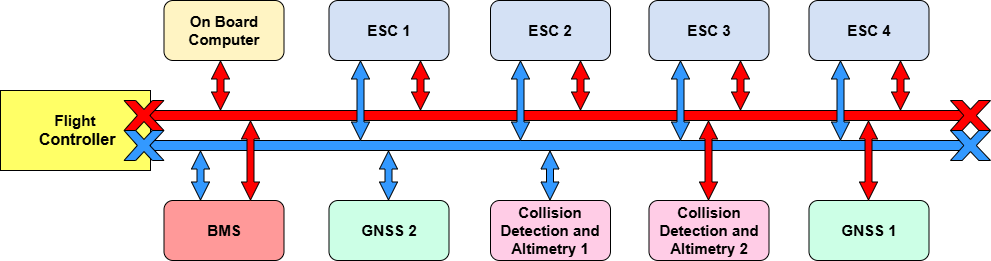
\includegraphics[width=1\textwidth]{figs/Thomas/Intra Communication/CAN bus.png}
 \caption{CAN bus layout}
 \label{fig:CAN_bus}
 \end{figure}

\subsubsection{Intra Board Selections}
\paragraph{\gls{IMU}}
As \gls{IMU}s provide key data for control and location sensing they should be used at the highest frequency possible. Frequencies greater than the control frequency are beneficial as you can use multiple data points to reduce the effect of white noise. Therefore, the simple but high speed \gls{SPI} protocol should be used. This is also a good option as \gls{SPI} is compatible with almost all modern \gls{IMU}s.
\paragraph{\gls{GNSS}}
\gls{GNSS} modules can communicate with \gls{UART} or \gls{I$^2$C}, both are simple and effective however, \gls{UART} is compatible with more modules and is therefore chosen.
\paragraph{Flight Controller MicroSD card}
MicroSD cards can communicate with \gls{SPI} or \gls{SDIO} as native. \gls{SDIO} is the native application and is faster and more effective, however, given the limited data transfer rates required and benefit of using \gls{SPI} over multiple devices and that on the selected \gls{MCU} a \gls{SWD} pin is also required for \gls{SDIO} means that using \gls{SPI} provided more benefit for the flight controller as the data transfer rates are well bellow the \textbf{SPI data limit}.
\paragraph{On Board Computer SD card}
As the data transfer rates are higher \gls{SDIO} becomes a required option as it can handle \textbf{a shittone of kilobytes} and we need \textbf{a shittone of kilobytes} which is over the \textbf{SPI data limit}.
\paragraph{\gls{LiDAR} Sensors}
\textbf{NEED specs from Huirui}
\paragraph{Imaging sensors}
The imaging sensors require high data transfer rates \textbf{quote the one for thermal and for GPR}, this means connecting them via Ethernet to the onboard computer with a maximum threshold of \textbf{Some number} would be most appropriate.
\paragraph{Low Speed Sensors}
Low speed sensors including any thermometers, barometers do not require high frequency 
communications, more than 1Hz, as these metrics do not change rapidly. This means that the lowest complexity and cost option, \gls{I$^2$C} should be used.
\paragraph{Debugger}
Debugging is possible using the \gls{CAN} bus at a system level but for in depth on board debugging that might be required for failure analysis or uploading code to boards should also be available. This can be done using \gls{UART} however, it is slower and has less functionality than using a \gls{SWD}. \gls{SWD} allows for real-time variable inspection and breakpoints. Therefore, for system wide debugging the \gls{CAN} bus will be used, and for onboard debugging a \gls{SWD} will be used.

\subsubsection{High Level Application Protocol}
\paragraph{Relevance}
A single high level protocol being used across all components makes the drone more adaptable and makes hiring developers easier. This is because a single skill-set can interact with the entire system. This however, comes with challenges due to the mapping sensors operating on different hardware to the other modules.
\paragraph{Cyphal}
Cyphal provides the perfect solution for this as it can be used over all major communication hardware. It was originally developed for, and is compatible with, \gls{UAV} components, and has since expanded to include further functionalities including Ethernet and \gls{USB}. This ensures that the system is easier to upgrade.
